\documentclass[reprint,amsmath,amssymb,aps,prd,nofootinbib,floatfix]{revtex4-2}

\usepackage{graphicx}
\usepackage{bm}
\usepackage{physics}
\usepackage{placeins}
\usepackage[nopatch=footnote]{microtype}

% Reduce minor underfull/overfull boxes without manual line-breaking
\setlength{\emergencystretch}{2em}

\begin{document}

\title{Minimal Point-Valued Stochastic Dynamics with Relaxing Memory: Markov Embedding and Metastable Structures}

\author{H. Horn}
\affiliation{Peine Stederdorf, Germany}

\date{28 February 2026} % explicit date for submissions/arXiv

\begin{abstract}
We propose a minimal point-valued stochastic dynamics on an abstract continuous state space $\Omega$ in which a visible trajectory $x_n$ is coupled to an explicit, exponentially relaxing memory density $\rho_n$.
The marginal process $\{x_n\}$ is generally non-Markovian, while the augmented state $z_n=(x_n,\rho_n)$ is Markov by construction.
The memory update is history-compressing, yielding an intrinsic arrow of \emph{update order}.
Coarse-graining over the internal persistence scale $n\gg\alpha^{-1}$ motivates an effective parameter $t=\alpha n$ and, when a separation of scales is present, an approximate continuum SDE/Fokker--Planck description.
In this regime we define trajectory-based, coordinate-robust diagnostics (persistence/relaxation rates, dimensionless stability measures, and metastable residence-time statistics) to identify and compare long-lived localized dynamical structures induced by the endogenous memory coupling.
Calibration to spacetime units, physical mass scales, relativistic dynamics, or Standard-Model-like structures is outside the scope of the present paper.
\end{abstract}

\maketitle

%-------------------------------------------------
\section{Introduction}
%-------------------------------------------------

Modern fundamental physics rests on a small number of highly successful theoretical frameworks, in particular quantum field theory and general relativity.
Despite their empirical success, both rely on foundational structures---spacetime, quantum states, and fields---that are postulated rather than derived.

This becomes particularly apparent in attempts to unify quantum theory and gravitation.
A range of non-perturbative programs (e.g., asymptotic safety \cite{Weinberg1979,Reuter1998,NiedermaierReuter2006,Percacci2017}, causal sets \cite{Bombelli1987,Sorkin2003}, loop-based formulations \cite{Rovelli2004,AshtekarLewandowski2004}, and string theory \cite{Polchinski1998}) achieves internal consistency but typically assumes notions such as time, locality, or dimensionality from the outset \cite{Anderson1972,Laughlin2000}.

The present paper is motivated by the hypothesis that these difficulties are not primarily technical, but conceptual.
Rather than postulating spacetime, quantum structure, or particles, we ask how such notions could arise from a more primitive irreversible dynamics.
Concretely, we assume only a sequence of non-trivial update events defining a trajectory in an abstract state space.

Related ideas appear in digital-physics approaches \cite{Wolfram2002,tHooft2016} and in history-dependent random-walk models \cite{Nelson1966,Pemantle2007,BenAImRaimond2002}.
Closest in spirit are self-interacting walks biased by their visitation history, such as the true (myopic) self-avoiding walk (TSAW) \cite{AmitParisiPeliti1983,TothWerner1998} and the self-repelling Brownian polymer (SRBP) \cite{DurrettRogers1992}; see also \cite{PelitiPietronero1987}.
Recent work on self-interacting diffusions continues to analyze processes whose drift depends on occupation-type memory variables \cite{HolbachRaimond2026}.

The second relevant strand is the use of Markovian embeddings for systems with memory.
For finite memory, the basic mechanism is elementary: one enlarges the state until the retained past is part of the present state.
Related embedding ideas also appear in generalized Langevin and nonlocal-memory equations, where auxiliary variables or spectral representations turn nonlocal memory terms into local evolution in an extended space \cite{NoeNuske2013,NoeWuPrinzPlattner2013,JaganathanValani2025,WisniewskiLuczkaSpiechowicz2024}.

Our model shares with self-interacting processes the idea of a trajectory coupled to a self-generated field, but differs structurally: the memory is an explicit, exponentially relaxing distribution updated by Eq.~(\ref{eq:memorydistribution}).
Consequently, the visible coordinate $x_n$ alone is generally non-Markovian, since its next update depends on the retained memory field, whereas the augmented state $z_n=(x_n,\rho_n)$ is Markov by construction.
This Markov embedding is the main mathematical anchor of the present paper.
The same memory update is information-losing at the level of histories and thereby induces an intrinsic arrow of \emph{update order} in the update dynamics; that is, in general the full ordered past cannot be reconstructed from the present state.
(We intentionally distinguish this update-order arrow from any thermodynamic or relativistic notion of physical time, which is not assumed here.)
Memory and trajectory thus emerge jointly as the minimal departure from trivial dynamics, rather than being encoded in external boundary conditions.

By contrast, TSAW/SRBP-type formulations are typically written directly in terms of the full occupation history (or local time) without explicit forgetting \cite{AmitParisiPeliti1983,TothWerner1998,DurrettRogers1992,PelitiPietronero1987}.
The broader placement of this construction within self-interacting diffusions, self-repelling polymers, Markovian embeddings of memory processes, and positive-operator formulations of stochastic maps is a natural subject for a separate mathematical companion note; the present paper keeps only the model definition and operational diagnostics needed for the minimal construction.

\paragraph{Roadmap (conceptual to operational).}
We first give a brief motivation (without a formal proof) for why a locally linear, metric-like coarse-grained description is a natural effective description once one assumes only directed, comparable update steps (Sec.~\ref{sec:minimalist_motivation}); readers primarily interested in the model and diagnostics may skip directly to Sec.~\ref{sec:MinDynModel}.
In Sec.~\ref{sec:MinDynModel} we specify the minimal generator---a point-valued stochastic update on $\Omega$ coupled to a relaxing memory distribution.
Sec.~\ref{sec:EffectiveTime} introduces an effective coarse-grained time parametrization and discusses when a continuum description is useful.
Subsequent sections analyze memory-induced irreversibility and then develop operational diagnostics (metastability, persistence/relaxation rates, and dimensionless stability measures) for robust, typically metastable dynamical structures.

A small reference implementation accompanies this work in the project repository and includes a relaxing-memory simulator, diagnostic functions, tests, and a reproducible reference runner.

%-------------------------------------------------
\subsection{Minimalist motivation: from directed updates to effective geometry}\label{sec:minimalist_motivation}
%-------------------------------------------------

Our starting point is deliberately weak: we assume only (i) distinguishable events and (ii) a directed update order between them.
To compare elementary updates, we further assume that minimal transitions can be assigned increments $\Delta$ in some comparison set $\mathcal{S}$ and that concatenation of transitions induces an associative composition law.

The purpose of this subsection is to justify why it is reasonable to work with continuum notions later on.
Under mild regularity and coarse-graining assumptions---continuity, refinement invariance, and a central-limit-type scaling of fluctuations---a consistent composition law can linearize locally and yield a tangent-space-like description.
If fluctuations are approximately isotropic at the coarse-grained scale, the covariance further induces an effective inner product.
In short: differentiability and metric structure are treated as \emph{effective} notions arising from stable large-scale behavior, not as fundamental axioms.

In the present paper we therefore work directly with a concrete minimal dynamics on a continuous state space $\Omega$.
The emergent coarse-grained geometry serves only as a consistency target and an interpretive guide for diagnostics extracted from trajectories.

%-------------------------------------------------
\section{Minimal Dynamical Model}\label{sec:MinDynModel}
%-------------------------------------------------

In this section we define the minimal dynamical framework underlying the present paper.
No assumptions about spacetime, physical geometry, quantum mechanics, physical fields, or conserved quantities are made at this stage.

\subsection{Background structure and invariances}\label{sec:background_invariances}

The model is formulated on a continuous state space $\Omega$ equipped with a reference measure $dx$ and a choice of local coordinates sufficient to define integrals and derivatives.
In practice one may take $\Omega\subseteq\mathbb{R}^d$ with the Lebesgue measure and the Euclidean inner product.
This background structure is a minimal mathematical scaffold for writing the generator and the diagnostics; it is not assumed to be a fundamental physical spacetime metric.

Two distinct notions of ``invariance'' are relevant.
First, once the extended state is defined in Eq.~(\ref{eq:augmented_state}), the resulting process is Markov by construction, and the update order $n\mapsto n+1$ is dynamically meaningful because the relaxing memory state compresses the ordered past.
Second, many of the observables we use are designed to be operational and robust under benign reparametrizations of $\Omega$ (e.g., translations, rotations, and global rescalings in the chosen coordinate chart), in the sense that they depend on coarse-grained residence statistics and relaxation rates rather than on absolute coordinate values.

Quantities that explicitly use $\nabla$ (e.g., drifts of the form $-\nabla\Phi[\rho]$ and Hessian-based OU linearizations) depend on the chosen coordinate/inner-product structure and should be interpreted as part of the effective description.
Accordingly, whenever we invoke ``isotropy'' or compare rates across runs, we do so at the level of dimensionless ratios or fit parameters extracted from trajectory data, not by assuming a preferred physical metric on $\Omega$.

\subsection{State and update index}

We consider a single generative process producing a sequence of states indexed by an integer update parameter $n\in\mathbb{N}$.
The parameter $n$ labels successive update steps of the process and does not represent physical time.

The full process state at update step $n$ is
\begin{equation} \label{eq:augmented_state}
z_n := (x_n,\rho_n).
\end{equation}

Here $x_n\in\Omega$ denotes the current position of the process, while $\rho_n$ is a memory density on $\Omega$ encoding the influence of past states.
The normalization condition specified below fixes the scale of the memory density and should not be read as an epistemic probability unless explicitly stated.
Given $z_n$ and a fresh noise draw $\xi_n$, the distribution of $z_{n+1}$ is determined by Eqs.~(\ref{eq:trajectory}) and~(\ref{eq:memorydistribution}).
This Markov embedding, summarized in Fig.~\ref{fig:markov_embedding}, is the Markovian description used throughout this paper.
The projected process $\{x_n\}$ alone is generally non-Markovian, because two identical visible positions with different memory densities can generate different next-step distributions.

Assumptions on $\Omega$ (continuity, reference measure, and coordinate/inner-product scaffold) were fixed in Sec.~\ref{sec:background_invariances} and are used here as an effective parametrization for writing Eqs.~(\ref{eq:trajectory})--(\ref{eq:memorypotential}). Throughout this paper, $\Omega$ remains an abstract state space; any identification with physical space or spacetime geometry is deferred to companion work.

The analysis below focuses on a single generative process.
This is sufficient for the Markov embedding, the memory-induced arrow of update order, and the metastability diagnostics developed here.
Coupled multiple generators, for example through a shared memory field, are a natural extension but are not required for the construction in this paper.

\subsection{Markov kernel and observable dynamics}

Let $\Sigma$ denote the augmented state space of pairs $z=(x,\rho)$.
To make the Markov embedding explicit, and to fix the operator language used later for relaxation and metastability, we represent the one-step stochastic update by a transition kernel rather than by a deterministic map:
\begin{equation}
P(z,A)
:=
\mathbb{P}\{z_{n+1}\in A\mid z_n=z\},
\qquad
A\subseteq\Sigma .
\end{equation}
Equivalently, the dynamics acts on bounded observables $f:\Sigma\to\mathbb{R}$ through the Markov/Koopman operator
\begin{equation}\label{eq:observable_operator}
(Uf)(z)
:=
\int_\Sigma f(z')\,P(z,dz')
=
\mathbb{E}[f(z_{n+1})\mid z_n=z].
\end{equation}
This operator is linear, positive, and unital ($U1=1$), while the dual operator propagates probability measures on $\Sigma$.
The iterates satisfy the semigroup relation $U^{m+n}=U^mU^n$.
In the stochastic case $U$ is generally not multiplicative, i.e. $U(fg)$ need not equal $(Uf)(Ug)$; hence the appropriate present language is a positive Markov operator on an observable algebra, not a deterministic automorphism of that algebra.
For compact or otherwise suitably topologized state spaces, closely related algebraic formulations identify stochastic maps with positive unital maps on commutative $C^*$-algebras, or more generally with morphisms in Markov categories \cite{Parzygnat2017,Fritz2020}.
This operator viewpoint is also the one used in transfer-operator and Koopman-based analyses of stochastic dynamics \cite{WilliamsKevrekidisRowley2015,KlusEtAl2018}.

This formulation also clarifies the sense in which the dynamics is irreversible.
For a fixed deposited kernel and $0<\alpha<1$, the affine update in $\rho$ can be algebraically rearranged, but the current augmented state does not retain the full ordered history and the stochastic kernel does not define a reversible group action in general.
The forward update order is represented by a Markov semigroup.

\subsection{Why a point-valued state? (minimal carrier choice)}

The fundamental dynamical variable $x_n$ is chosen to be a single point in state space.
This is not meant as a physical claim that fundamental entities are point particles.
Rather, it is a minimal \emph{carrier} of sequential updates: any iterative generator must, at each step, select ``what happened'' in some configuration space, and a point-valued state is the simplest such representation.

Importantly, the formalism is not tied to this choice.
One may replace $x_n$ by (for example) a field configuration, a graph, a tuple of points, or a probability distribution; the same structural idea then becomes an irreversible update of a relaxing-memory variable coupled back into the generator.
We therefore view ``point'' as a design choice that makes the mechanism maximally transparent, not as an asserted inevitability.

In the baseline normalization used here, the memory variable $\rho_n(x)$ is a non-negative density (with respect to a chosen reference measure $dx$) with unit total weight,
\begin{equation}
\rho_n(x) \ge 0,
\qquad
\int_\Omega \rho_n(x)\,dx = 1,
\end{equation}
which we assume to be effectively localized (e.g., rapidly decaying outside a characteristic region).
This is a convenient scale convention rather than a fundamental postulate: it makes $M_n(\mathcal{K})$ a visitation/memory weight and leaves $\eta$ as the coupling strength to the memory-induced drift.
Equivalently, one could work with finite positive memory measures and absorb the total memory scale into $\eta$.
Implicitly, the unit-weight convention presumes either $\Omega=\mathbb{R}^d$ with sufficiently fast decay, or boundary conditions (e.g., periodic or reflecting) under which the update in Eq.~(\ref{eq:memorydistribution}) preserves total mass.

\subsection{Trajectory update rule}

The evolution of the position variable is governed by
\begin{equation}\label{eq:trajectory}
x_{n+1} = x_n + \varepsilon\,\xi_n - \eta\,\nabla\Phi_n(x_n).
\end{equation}

The appearance of $\nabla$ should be read as an effective smooth structure tied to the chosen coordinate chart on $\Omega$.
At the discrete level, one could equivalently replace the gradient by a local finite-difference/score-type rule on the coarse-graining scale $\sigma$; the use of $\nabla$ is a compact notation anticipating that the memory potential $\Phi_n$ is smooth once $\rho_n$ is a mixture of smooth kernels $G_\sigma$.
Thus, differentiability is not a fundamental assumption about ``spacetime,'' but a property of the coarse-grained interaction term induced by the memory update.

The stochastic variable $\xi_n$ is assumed to be isotropic and dimensionless, with unit variance \cite{Gardiner2009}. As in Sec.~\ref{sec:background_invariances}, ``isotropic'' is understood relative to the chosen coordinate/inner-product scaffold on $\Omega$, not as a fundamental physical postulate. The parameters $\varepsilon$ and $\eta$ control the relative strength of stochastic fluctuations and memory-induced drift.

\subsection{Memory update rule}
The memory distribution evolves according to
\begin{equation}\label{eq:memorydistribution}
\rho_{n+1}(x) = (1-\alpha)\rho_n(x) + \alpha\,G_\sigma(x-x_{n+1}),
\end{equation}
where $G_\sigma$ is a smooth, normalized kernel with finite width $\sigma$.
As an update of a full trajectory history into a single current density, this rule is history-compressing: the exponentially weighted past is represented by the current field $\rho_n$ rather than by retaining the full ordered history as a primitive object.
This memory-state embedding is what makes the model Markov in the augmented state.

\begin{figure}[!tbp]
    \centering
    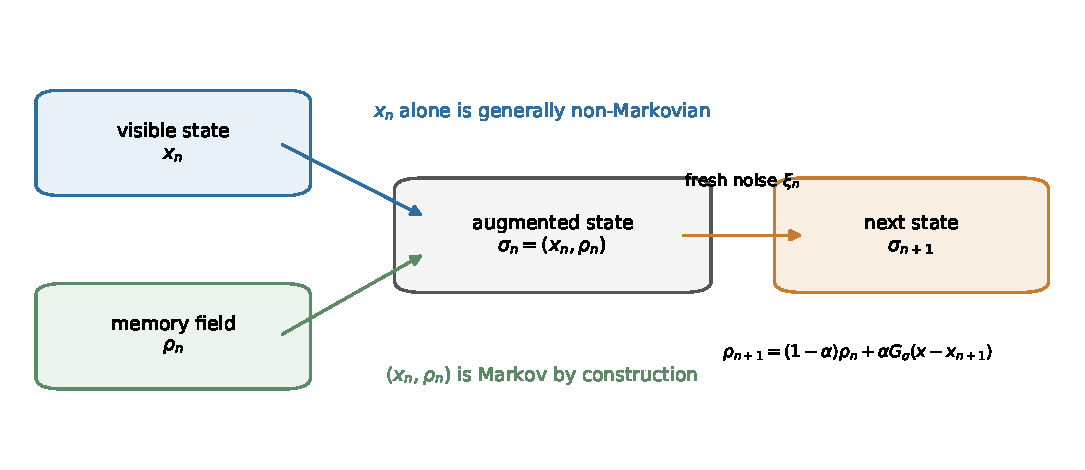
\includegraphics[width=\linewidth]{fig_markov_embedding.pdf}
    \caption{
    Memory-state Markov embedding.
    The visible coordinate $x_n$ is generally non-Markovian by itself, because the next update depends on the accumulated memory field $\rho_n$.
    Once $z_n=(x_n,\rho_n)$ is used as the state, all past influence enters through $\rho_n$, while fresh randomness enters through $\xi_n$.
    }
    \label{fig:markov_embedding}
\end{figure}

For definiteness, one may assume that $G_\sigma$ is radially symmetric and either compactly supported or rapidly decaying, so that it defines a controlled coarse-graining scale $\sigma$. Similarly, the interaction kernel $K(x,y)$ is assumed to be sufficiently smooth and (in typical examples) symmetric, $K(x,y)=K(y,x)$; translation-invariant choices $K(x,y)=K(x-y)$ provide a simple baseline class.

At the same time, the freedom in choosing $(G_\sigma,K)$ is substantial and defines a broad family of models. The existence of an intrinsic arrow of update order is tied to the history-compressing memory representation. By contrast, the detailed phenomenology of localization and knot formation depends on qualitative features of $K$ (e.g., symmetry, range, and effective repulsive/attractive character) and on how $G_\sigma$ sets the coarse-graining scale.

As a concrete baseline example (used in the numerical illustrations), one may take $G_\sigma$ to be a radially symmetric Gaussian kernel and choose a translation-invariant interaction kernel of the form $K(x,y)=K_\ell(x-y)$ with a single interaction length $\ell$.

\subsection{Memory potential}

The influence of memory on the trajectory is mediated by the potential
\begin{equation}\label{eq:memorypotential}
\Phi_n(x) := \int_\Omega K(x,y)\,\rho_n(y)\,dy,
\end{equation}
where $K(x,y)$ is a smooth interaction kernel. 
The integral form ensures a smooth, non-local influence of accumulated memory \cite{Mori1965,Zwanzig2001}.
The gradient in Eq.~(\ref{eq:trajectory}) acts on the first argument of the kernel: whenever differentiation under the integral is justified, $\nabla\Phi_n(x)=\int_\Omega \nabla_x K(x,y)\rho_n(y)\,dy$.
For a translation-invariant kernel $K(x,y)=K_\ell(x-y)$, this is the convolution of $\rho_n$ with $\nabla K_\ell$; it vanishes only in special cases such as locally constant kernels or symmetry-balanced memory configurations.

\subsection{Relaxing-memory sum form}

Although we write $\rho_n$ as a density and $\Phi_n$ as an integral, iterating Eq.~(\ref{eq:memorydistribution}) shows that $\rho_n$ is an explicitly computable, exponentially weighted mixture of kernels centered on past positions.
Equivalently, $\Phi_n$ can be evaluated as the corresponding weighted superposition of kernel responses.
The resulting age weights are shown in Fig.~\ref{fig:memory_weights}; the continuum notation is only a compact representation of this discrete, relaxing-memory mechanism.

\subsection{Parameters and scaling}
The model is characterized by three parameters $\varepsilon$, $\eta$, and $\alpha$, which set the scales of stochastic displacement, memory-induced drift, and memory relaxation, respectively. No physical interpretation is assigned to these parameters at this stage.

\paragraph{Parameter conventions.}
Throughout, $\varepsilon$ sets the typical stochastic displacement per update step (noise amplitude), $\eta$ sets the strength of the memory-induced drift, and $\alpha\in(0,1]$ controls the memory relaxation rate (effective persistence length $\sim\alpha^{-1}$ updates). The kernel width $\sigma$ defines the coarse-graining scale of the memory update, and $\ell$ (when used) denotes an interaction length scale entering the kernel $K_\ell$.

\subsection{Explicit non-assumptions}

We do not assume spacetime, quantum postulates, physical fields, physical symmetries, or conservation laws; these are treated as structures to be recovered, if at all, only in an effective description.


%-------------------------------------------------
\section{Irreversible Memory and Effective Time}
%-------------------------------------------------

The defining feature of the model in Sec.~\ref{sec:MinDynModel} is a self-interacting, exponentially relaxing memory.
Irreversibility here does not mean thermodynamic entropy production; it means loss of ordered-history information under compression into the current memory state.
We therefore work with the update index $n$ and the ordered state sequence $z_n$.

\subsection{Information compression and update order}

Equation~(\ref{eq:memorydistribution}) represents the ordered past by a compressed density: new contributions are added locally, while older contributions are exponentially suppressed.
For fixed $x_{n+1}$ and $0<\alpha<1$, the equation is algebraically invertible as an affine map in $\rho_n$, but this inverse does not recover the discarded ordered trajectory history.
The structural many-to-one map is from ordered histories to the current memory density.
Thus $\rho_n$ stores cumulative influence rather than a sequence of past positions, and multiple distinct histories may lead to the same present state even without noise in Eq.~(\ref{eq:trajectory}).
This information compression gives dynamical relevance to the update ordering.
The state sequence in Eq.~(\ref{eq:augmented_state})
\[
z_0 \rightarrow z_1 \rightarrow z_2 \rightarrow \dots
\]
acquires an intrinsic, irreversible ordering without assuming spacetime or calibrated physical time.

\subsection{Role of the memory rate}

Figure~\ref{fig:memory_weights} makes the role of $\alpha$ explicit: it controls how long past updates remain dynamically active.
Small $\alpha$ produces long memory and extended correlations; larger $\alpha$ suppresses older contributions more quickly and favors more transient structures.
The qualitative consequences of this persistence scale become visible in the knot trajectories of Fig.~\ref{fig:3d_knot_trajectory}.

\begin{figure}[!tbp]
    \centering
    
\includegraphics[width=\linewidth]{fig_memory_weights.pdf}
    \caption{
    Exponential memory weights generated by Eq.~(\ref{eq:memorydistribution}).
    A contribution of age $m$ enters with weight $w_m=\alpha(1-\alpha)^m$.
    When ages are measured in the scaled variable $\alpha m$, the accumulated memory weight collapses onto a persistence scale of order $\alpha^{-1}$ updates.
    }
    \label{fig:memory_weights}
\end{figure}

\subsection{Effective time (coarse-graining)}\label{sec:EffectiveTime}

Although the update index $n$ is not physical time, the history-compressing memory dynamics makes the ordering of updates dynamically relevant.
The memory update rule Eq.~(\ref{eq:memorydistribution}) introduces a natural persistence scale of order $\alpha^{-1}$ update steps, which sets the coarse-graining resolution.
In regimes where coarse observables vary slowly on this scale, we use the effective (dimensionless) parameter
\begin{equation}\label{eq:t_taup}
t := \alpha n.
\end{equation}
Here $t$ counts (approximately) how many persistence scales have elapsed along the update sequence.
Correspondingly, since $\Delta t = \alpha$ per update step, differences in Eq.~(\ref{eq:trajectory}) may be approximated as
\begin{equation}
\frac{x_{n+1} - x_n}{\alpha}
\;\longrightarrow\;
\frac{\mathrm{d}x}{\mathrm{d}t}.
\end{equation}

This provides a convenient parametrization of the large-scale behavior of the discrete dynamics; different choices of coarse-graining correspond to different effective time resolutions.

We stress that $t$ is, at this stage, an auxiliary coarse-grained parameter and remains dimensionless unless an additional calibration is introduced.
Moreover, in a strict continuum limit the discrete noise $\varepsilon\,\xi_n$ must be rescaled to yield a finite diffusion coefficient; a standard choice is a joint limit $\alpha\to 0$ and $\varepsilon\to 0$ at fixed $\varepsilon^2/\alpha$.

\subsection{Operational time scale}

The definition $t=\alpha n$ can be read purely as a reparametrization.
What makes it non-trivial in the present framework is that $\alpha^{-1}$ is not an externally supplied clock: it is an \emph{internally available} scale defined by the irreversible memory update, and it is operationally estimable from data of a single run (e.g., by the exponential forgetting rate of contributions to $\rho_n$).
In this sense, the continuum parameter $t$ is tied to a dynamical coarse-graining defined within the model, rather than being an independent fundamental input.

\subsubsection{Operational diagnostics}

This paper uses a small set of data-driven quantities for cross-run comparison:
\begin{itemize}
\item $\alpha$ is estimated from the memory-weight decay shown in Fig.~\ref{fig:memory_weights}, by fitting $(1-\alpha)^m\simeq e^{-\alpha m}$ or a memory-sensitive observable such as $\Phi[\rho_n](x_n)$.
\item $D$ is the effective diffusion coefficient of the coarse-grained dynamics, with the continuum-limit scaling specified in Eq.~(\ref{eq:coarse_sde}).
\item $\Gamma_{\mathrm{rel}}$ is the knot relaxation rate extracted from the decay of an in-knot autocorrelation $C(t)\propto e^{-\Gamma_{\mathrm{rel}} t}$ or from the dominant relaxation eigenvalue of a quasi-stationary local linearization.
\item $\widehat{\Gamma}$ is a dimensionless stability measure, defined below, that compensates for uniform coordinate rescalings of the effective state space.
\end{itemize}

These diagnostics are intended to be operational: they can be estimated from simulation trajectories without assuming an a priori physical time unit.

\paragraph{Estimating $\alpha$ (and thus $t$) from a single trajectory.}
Because the memory update is linear and relaxing, the contribution of an update at step $k$ to later memory states $\rho_n$ is exponentially suppressed for $n\!>\!k$.
For the canonical update rule
\begin{equation}\label{eq:rho_linear_solution}
\rho_{n}(x)=(1-\alpha)^{n-k}\rho_{k}(x)
+\alpha\sum_{j=k+1}^{n}(1-\alpha)^{n-j}\,G_\sigma(x-x_{j})
\end{equation}
the kernel contribution inserted at step $j$ has age $m:=n-j$ and weight $\alpha(1-\alpha)^m\simeq\alpha e^{-\alpha m}$ for $\alpha\ll 1$.
Operationally, one may therefore estimate $\alpha$ by fitting an exponential decay law in $n$ for any memory-sensitive observable (e.g., the autocorrelation of a local functional of $\rho_n$ or of the induced drift $-\nabla\Phi[\rho_n](x_n)$), and then set $t:=\widehat{\alpha}\,n$ for cross-run comparisons.

Comparability between independent realizations can then be achieved by matching such intrinsic, dimensionless decay laws, which fixes the unit of $t$ up to statistical uncertainty.

Formally, one may write the coarse-grained dynamics as a stochastic differential equation
\begin{equation}\label{eq:coarse_sde}
\mathrm{d}x = -\frac{\eta}{\alpha}\,\nabla\Phi[\rho(t)](x)\,\mathrm{d}t + \sqrt{2D}\,\mathrm{d}W_t,
\qquad
D \sim \frac{\varepsilon^2}{2\alpha},
\end{equation}
where $W_t$ is a standard Wiener process \cite{Oksendal2003,Risken1996}. We emphasize that the potential is induced by the memory field, $\Phi[\rho](x):=\int K(x,y)\rho(y)\,dy$, and is therefore slowly time-dependent in general.
In metastable knot regimes it may be treated as quasi-stationary on intermediate time scales. The precise numerical prefactor depends on conventions and on how the discrete-to-continuum limit is taken.

Unless stated otherwise, SDEs are interpreted in the It\^o sense.


\paragraph{Temporal direction and limits}
Because the memory update compresses the ordered past, the coarse-grained parameter $t$ inherits a preferred direction: reversing $t$ does not correspond to a valid evolution of the discrete process.
Moreover, $t$ is useful only when memory relaxation provides a separation of scales.
For $\alpha\to 1$ memory becomes too short-lived for a controlled continuum description, while for $\alpha\to 0$ memory persists over arbitrarily long sequences and the coarse-graining becomes ambiguous.

In the regimes where a continuum description is meaningful, the next question is whether the dynamics self-organizes into robust metastable regions $\mathcal{K}\subset\Omega$.
We identify such ``dynamical knots'' operationally via the memory/visitation measure $M_n(\mathcal{K})$ and characterize their stability by an associated relaxation rate $\Gamma_{\mathrm{rel}}$.

%-------------------------------------------------
\section{Dynamical Knots and Relaxation Scales}
%-------------------------------------------------

Having established an effective notion of time, we now turn to memory-induced localized structures and their relaxation-based mass-like proxy.

\subsection{Dynamical knots}

As illustrated in Fig.~\ref{fig:3d_knot_trajectory}, the trajectory generated by the update rules may organize into localized regions of repeated visitation.
These regions are not imposed externally, but arise dynamically through the interplay of
stochastic motion and memory-induced drift.

We refer to such regions as \emph{dynamical knots}.
A dynamical knot is characterized by an enhanced local memory density Eq.~(\ref{eq:memorydistribution}) and a corresponding self-consistent modification of the trajectory dynamics.
Importantly, a knot is not an object or a fixed point, but a metastable dynamical pattern.
Operationally, a knot may be identified by a metastable region $\mathcal{K}\subset\Omega$ with coarse-grained visitation measure (equivalently, memory weight)
\begin{equation}
M_n(\mathcal{K}) := \int_{\mathcal{K}}\rho_n(x)\,dx
\end{equation}
Persistence means that $M_n(\mathcal{K})$ remains above a chosen threshold over update intervals $\Delta n \gg \alpha^{-1}$.

Here $M_n$ is a region-level observable, while the induced potential $\Phi_n(x)=\int K(x,y)\rho_n(y)\,dy$ is a field on $\Omega$.
Intuitively, elevated $M_n(\mathcal{K})$ means that $\rho_n$ carries substantial weight near $\mathcal{K}$; through the convolution with $K$, this can generate a locally restoring drift $-\nabla\Phi_n$ that stabilizes the knot.

This trajectory-level definition is deliberately minimal, but it has a direct operator-theoretic refinement.
Once augmented features along the trajectory are recorded, a chosen lag and a coarse partition or basis on $\Sigma$ define an estimated transfer operator.
Candidate knots can then be tested as metastable or almost-invariant sets, equivalently as slowly decaying modes separated by a spectral gap \cite{FroylandLloydSantitissadeekorn2010,NoeNuske2013}.
The present paper uses residence weights and relaxation fits as the minimal diagnostic version of this criterion; a full transfer-operator/MSM analysis is left to subsequent work.

\begin{figure}[!b]
    \centering
    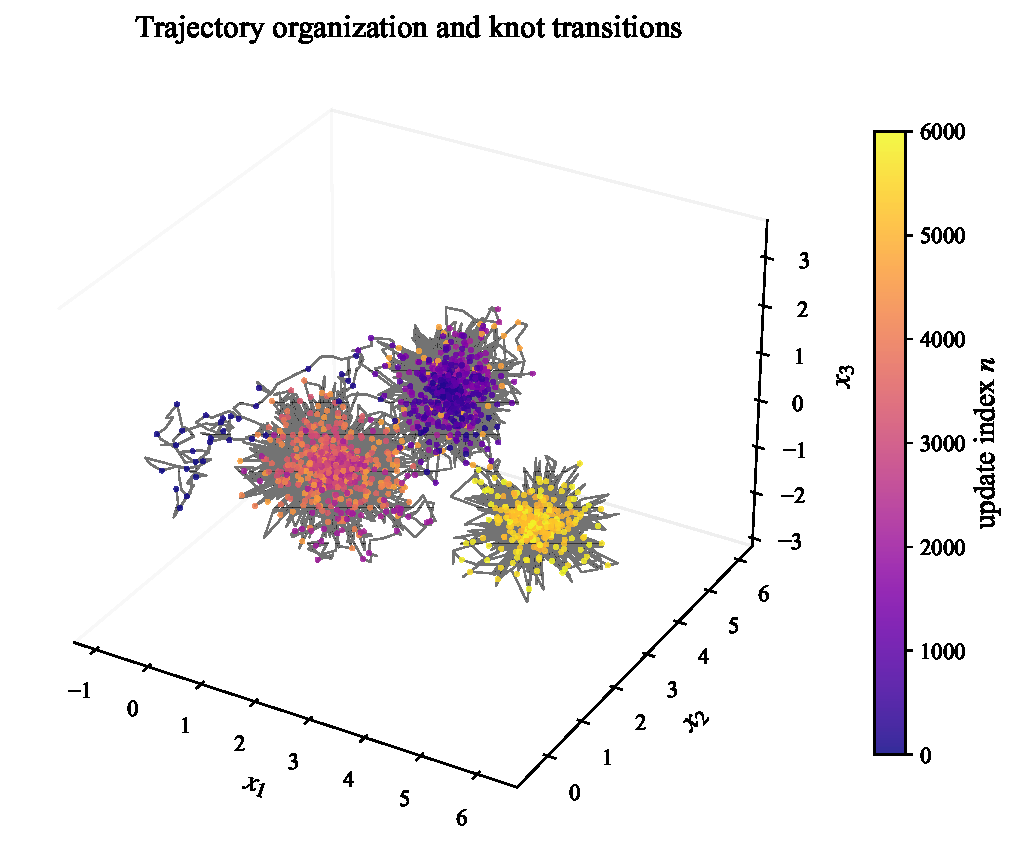
\includegraphics[width=0.88\linewidth]{fig3_knot_trajectory.pdf}
    \caption{
    Organization of a trajectory into multiple knot-like regions in state space.
    The continuous line shows the full trajectory, while discrete points indicate sampled positions
    contributing to the memory distribution.
    Color denotes the update index $n$.
    Shown is a representative run illustrating metastable clustering in one parameter regime.
    }
    \label{fig:3d_knot_trajectory}
\end{figure}

In such regimes, the coarse-grained dynamics typically exhibits two distinct time scales: the memory persistence scale of order $\alpha^{-1}$ and a (potentially larger) knot relaxation scale $\tau_{\mathrm{rel}}$ characterizing return to the metastable region after perturbations.
Operationally, $\tau_{\mathrm{rel}}$ is defined with respect to the coarse-grained parameter $t$ (Sec.~\ref{sec:EffectiveTime}), e.g., by an exponential decay law of an in-knot autocorrelation $C(t)\propto e^{-t/\tau_{\mathrm{rel}}}$.
This motivates using a relaxation rate (and its dimensionless variant) as an operational descriptor of knot stability.

\subsection{Attractors of the effective dynamics}

In the continuum description, the influence of memory may be summarized by an effective potential $\Phi[\rho](x)$ induced by the memory field.
In a frozen-memory approximation, dynamical knots can be represented locally by regions where the gradient of this potential vanishes,
\begin{equation}
\nabla \Phi[\rho](x_\star) = 0,
\end{equation}
and small perturbations are suppressed. In the presence of stochastic forcing, knots are typically metastable (noise-broadened) attractor regimes rather than strictly stable fixed points.

In this approximation, the Hessian of the memory potential defined in Eq.~(\ref{eq:memorypotential}) determines the local relaxation rates.
Linearizing the continuum drift corresponding to Eq.~(\ref{eq:trajectory}) around such a point $x_\star$ yields an OU-type approximation,
\begin{equation}
\mathrm{d}x = -\gamma H (x - x_\star)\,\mathrm{d}t + \sqrt{2D}\,\mathrm{d}W_t,
\end{equation}
where $H$ denotes the Hessian of the memory potential evaluated at $x_\star$, and
\begin{equation}
\gamma := \frac{\eta}{\alpha}
\end{equation}
collects the effective coupling to the memory-induced drift in the continuum description.

\paragraph{Remark (stability condition and time dependence).}
Strictly, $x_\star$ is a fixed point only for a \emph{frozen} memory field (i.e., if $\rho$ is quasi-stationary on the relaxation time scale).
Local stability in the linearized (OU) approximation requires the symmetric part of $H$ to be positive definite (so that the drift is restoring) in the directions of interest; otherwise $x_\star$ is unstable or saddle-like and does not define a metastable knot.

This form describes a relaxation process toward the attractor, with characteristic decay
rates determined by the eigenvalues of $H$ \cite{Strogatz2018}.
If $\lambda$ denotes a characteristic restoring eigenvalue of $H$, the associated relaxation rate scales as
\begin{equation}
\Gamma_{\mathrm{rel}} \sim \frac{\eta}{\alpha}\,\lambda.
\end{equation}

\subsection{Mass-like proxy as relaxation scale}

The stability of a dynamical knot is governed by the rate at which perturbations decay.
We therefore associate the mass-like scale of a knot not with resistance to acceleration, but with a relaxation scale characterizing the response of the system to fluctuations.

Concretely, in the coarse-grained (Markovian) regime one may define a characteristic relaxation time $\tau_{\mathrm{rel}}$ from linear response, e.g., from the decay of the autocorrelation of $x(t)$ within a metastable region.
Locally, $\tau_{\mathrm{rel}}$ can be obtained from the spectral gap of the linearized Fokker--Planck generator around the knot.
Globally, the same diagnostic is naturally phrased in terms of slow eigenvalues of a lagged transfer operator.
Figure~\ref{fig:relaxation_diagnostic} shows the corresponding trajectory-level diagnostic.
It is then natural to work with the associated relaxation rate
\begin{equation}
\Gamma_{\mathrm{rel}} := \frac{1}{\tau_{\mathrm{rel}}},
\end{equation}
with ``heavier'' knots corresponding to larger $\Gamma_{\mathrm{rel}}$ (faster relaxation, stronger confinement against fluctuations).
In a transfer-operator description at lag $\tau$, a slow eigenvalue $\mu_i(\tau)$ gives the rate
\begin{equation}
\Gamma_i(\tau) := -\frac{1}{\tau}\log|\mu_i(\tau)|,
\end{equation}
with small $\Gamma_i$ corresponding to slowly relaxing modes.
The local Hessian formula above is therefore best read as a quasi-stationary, local approximation to this broader spectral diagnostic.

For coordinate-scaling robustness, one may report a dimensionless version using the intrinsic coarse-graining scales $\sigma$ and $D$ of the continuum description,
\begin{equation}
\widehat{\Gamma} := \frac{\sigma^2}{D}\,\Gamma_{\mathrm{rel}}.
\end{equation}
In knot regimes where a quasi-stationary linearization is valid, one expects $\Gamma_{\mathrm{rel}}$ to track the Hessian eigenvalue scale of the local attractor, up to convention-dependent numerical factors.
Moreover, under a uniform rescaling of coordinates $x\mapsto a x$ (with corresponding rescalings of the coarse-graining width $\sigma$), the dimensionless quantity $\widehat{\Gamma}$ should remain approximately invariant.
A sharper identification with a physical mass scale requires (and is deferred to later work) an emergent geometric calibration and an operational mapping to energy units.

\begin{figure}[!tbp]
    \centering
    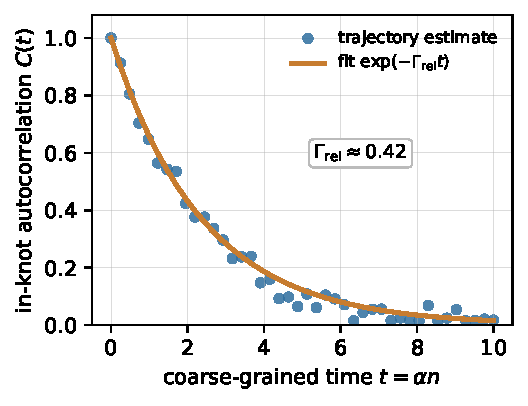
\includegraphics[width=0.58\linewidth]{fig_relaxation_diagnostic.pdf}
    \caption{
    Operational extraction of a knot relaxation rate from an in-knot autocorrelation.
    The decay of a coarse-grained observable $C(t)$ over the intrinsic parameter $t=\alpha n$ defines $\tau_{\mathrm{rel}}$ and hence $\Gamma_{\mathrm{rel}}=1/\tau_{\mathrm{rel}}$.
    The figure is schematic: the diagnostic is the fitted relaxation scale, not the specific numerical value.
    }
    \label{fig:relaxation_diagnostic}
\end{figure}

\paragraph{Terminology (``mass'' as an operational proxy).}
We stress that ``mass'' here is not meant as a postulated inertial parameter of a background spacetime.
Rather, it is a coarse-grained, quasi-time-independent property of a metastable attractor regime, quantified by how rapidly perturbations relax back into the knot.
The terminology is therefore intentionally closer to ``stiffness'' or ``confinement strength'' than to Newtonian inertia; a mapping to conventional energy/mass units requires an additional calibration and is deferred to companion work.

\subsection{Metastability and transitions}

Not all knots are permanently stable.
Depending on the memory rate $\alpha$ and the strength of stochastic fluctuations, knots
may be metastable and decay over long but finite times \cite{Kramers1940,FreidlinWentzell2012}.
Transitions between different knot configurations correspond to qualitative changes in
the organization of the trajectory.

Such transitions are evident in Fig.~\ref{fig:3d_knot_trajectory}, where the trajectory
moves between distinct regions of enhanced memory feedback.
These processes provide a minimal setting for studying transition-like events in effective dynamics at larger scales.

\subsection{Dimensionless diagnostics and effective scales}

The minimal dynamical model introduced in Sec.~\ref{sec:MinDynModel} is defined in terms of three parameters, $\varepsilon$, $\eta$, and $\alpha$, which characterize stochastic fluctuations, memory-induced drift, and memory relaxation, respectively.
We now summarize the effective scales and, crucially, dimensionless combinations that serve as operational diagnostics within the coarse-grained description.
A calibration of these scales to familiar physical constants and units is deferred to companion work.

\subsection{Diffusion and relaxation scales}

As fixed by the coarse-grained SDE in Eq.~(\ref{eq:coarse_sde}), the stochastic contribution is summarized by the effective diffusion constant $D$, up to convention-dependent numerical factors.
Together with the knot relaxation rate $\Gamma_{\mathrm{rel}}$, the pair $(D,\Gamma_{\mathrm{rel}})$ forms a minimal set of effective scales that organize the metastable regimes analyzed here.

The dimensionless diagnostic $\widehat{\Gamma}$ compares relaxation to diffusion on the coarse-graining scale and is approximately invariant under uniform coordinate rescalings $x\mapsto a x$ (with corresponding rescaling of $\sigma$).

A useful control ratio may then be defined as $R:=\Gamma_{\mathrm{rel}}/\Delta\Gamma$, where $\Delta\Gamma$ denotes the fluctuation-induced uncertainty of the relaxation estimate across windows or realizations.
Here, $R$ is only an operational drift-to-fluctuation diagnostic; a fuller phase-level interpretation is deferred to companion work.

\subsection{Diffusive relaxation scale}

The local linearization links the operational relaxation diagnostic of Fig.~\ref{fig:relaxation_diagnostic} to the Hessian eigenvalue scale of the effective attractor dynamics.

Since no metric is assumed on $\Omega$, the numerical value of $\lambda$ depends on the coordinate scaling of the state space. In practice, the kernel width $\sigma$ provides a natural reference scale, allowing one to form a dimensionless curvature measure $\tilde{\lambda} := \sigma^2\lambda$.

To summarize relaxation and stochastic broadening without introducing additional postulates in the present paper, one may form the product
\begin{equation}
Q_{\mathrm{rel}} \;:=\; 2D\,\Gamma_{\mathrm{rel}},
\end{equation}
which is controlled by the same two coarse-grained quantities that already appear in the OU approximation and in the dimensionless stability measure $\widehat{\Gamma}$.
A later calibration may determine whether a suitably normalized version of $Q_{\mathrm{rel}}$ can be interpreted as an energy-like scale; that identification is not assumed here.

In this formulation, the mass-like proxy is not a fundamental parameter but a measure of the stability of an attractor against stochastic perturbations.
Heavier structures correspond, operationally, to steeper memory-induced potentials and/or stronger memory coupling, and thus faster relaxation.

%-------------------------------------------------
\section{Discussion and Outlook}
%-------------------------------------------------

We introduced a minimal self-interacting point-valued stochastic dynamics with exponentially relaxing memory.
The visible coordinate is generally non-Markovian, while the augmented state $(x_n,\rho_n)$ gives a natural Markov embedding.
The history-compressing memory update induces an intrinsic arrow of \emph{update order} without assuming thermodynamic irreversibility, physical time, or spacetime structure.
Coarse-graining on the memory-persistence scale yields an effective integration parameter $t=\alpha n$ and, when a separation of scales is present, a useful continuum SDE/FP approximation.

Within this effective regime, the dynamics can self-organize into localized, long-lived metastable structures (``dynamical knots'').
Their stability can be quantified operationally via relaxation rates, dimensionless stability measures, and residence-time statistics extracted directly from trajectories.
Interpreting such stability scales as mass-like proxies is natural at the level of the effective description, while any identification with physical units and relativistic structure is deferred to companion work.

Several limitations and open directions remain.
The continuum description is used here as an effective approximation rather than as a proven scaling limit; a rigorous convergence analysis, including conditions on $(G_\sigma,K)$ and parameter scalings, is left for future work.
A small NumPy reference implementation, tests, and a reproducible reference runner provide a concrete basis for verifying the numerical diagnostics reported in this draft.
Finally, extending the framework to multiple coupled generators and exploring when consistent universal scales emerge are natural next steps.
From the algebraic viewpoint, a later stage can also ask which transformations preserve the transition kernel or its metastable sets.
Such stabilizer or equivariance structures would be the appropriate place to look for effective symmetry algebras; they are not assumed in the present minimal model.

\begin{acknowledgments}
The author thanks colleagues for valuable feedback and discussion.
\end{acknowledgments}

% Use a BibTeX style that avoids RevTeX's journal abbreviation list warnings (jnrlst)
\bibliographystyle{unsrtnat}
\bibliography{references}

\end{document}
